% MCQMC 2024 template files reused from the Aadit paper at Fred's request.
% Final MCQMC 2026 template compliance remains to be checked.
\documentclass{svproc}
\usepackage{amsmath,amssymb,mathtools}
\usepackage{newtxtext}
\usepackage[varvw]{newtxmath}
\usepackage{url}
\def\UrlFont{\rmfamily}
\usepackage{graphicx,booktabs,enumitem,xcolor}
\usepackage[hidelinks]{hyperref}
\usepackage{microtype}
\newcommand{\vx}{\boldsymbol{x}}
\newcommand{\vz}{\boldsymbol{\zeta}}
\newcommand{\vh}{\boldsymbol{h}}
\newcommand{\vDelta}{\boldsymbol{\Delta}}
\newcommand{\vzero}{\boldsymbol{0}}
\newcommand{\E}{\mathbb{E}}
\newcommand{\R}{\mathbb{R}}
\newcommand{\N}{\mathbb{N}}
\newcommand{\dif}{\,\mathrm{d}}
\newcommand{\fracpart}[1]{\{#1\}}
\newcommand{\kt}{\widetilde K}
\newcommand{\W}{\mathcal W}
\newcommand{\Hspace}{\mathcal H}
\newcommand{\fredcodex}[1]{{\color{red!70!black}#1}}
\newcommand{\codex}[1]{\begingroup\color{green!60!black}#1\endgroup}
\newcommand{\codexdone}[1]{\begingroup\color{gray}#1\endgroup}
\DeclareMathOperator*{\argmin}{arg\,min}
\title{Component-by-Component Constructions of Kronecker and Lattice Sequences Which Are Good for Arbitrary Sample Sizes}
\titlerunning{CBC sequences for arbitrary sample sizes}
\author{Alexander Pride \and Fred J. Hickernell}
\authorrunning{Alexander Pride and Fred J. Hickernell}
\institute{}
\date{October 28, 2026}
\begin{document}
\mainmatter
\maketitle
\begin{center}\small Discussion draft for Fred and Anders. MCQMC 2024 macros; limit: 16 pages.\end{center}
\begin{abstract}
Lattice rules are commonly constructed to perform well at sample sizes that
are powers of a fixed base. In applications, however, the available budget
may stop between these preferred sizes. We consider component-by-component
(CBC) constructions that optimize an aggregate of the expected squared
discrepancies of all prefixes up to a chosen horizon. The aggregate uses
sample-size weights distinct from the coordinate weights of the function
space. For base-two lattice sequences, dyadic difference multiplicities
reduce the criterion to a weighted kernel sum. A reversed digit-permutation
scrambling, called Newo, leaves every prefix's shift-averaged squared
discrepancy unchanged when applied to the scalar van der Corput sequence
before multiplication by a fixed lattice generator. We present a direct
permutation proof and its implication for CBC construction. For Kronecker
sequences, a lag-based expression yields a related CBC objective. Historical
comparisons from the special-session talk motivate the construction; the
numerical study and the newer Kronecker algorithm remain under development.
\keywords{quasi-Monte Carlo, lattice sequence, Kronecker sequence,
component-by-component construction, arbitrary sample size, scrambling.}
\end{abstract}

\par\smallskip
\noindent\codex{[Revision later: Revise the abstract after the newer Kronecker
construction and final experiments are in place. The present abstract describes
a discussion draft, not the final submission's completed contributions.]}
\par\smallskip

\section{Introduction}\label{sec:introduction}
An integration algorithm may be interrupted when its budget is exhausted,
when another simulation finishes, or when an error diagnostic indicates
sufficient accuracy. There is no reason for that stopping point to coincide
with a power of two. This motivates a construction problem for entire
sequences: choose one generator whose successive prefixes have small
integration errors over a range of sample sizes, rather than optimize only
a distinguished terminal point set.

For an integrand $f:[0,1)^d\to\R$, write
\[
 I(f)=\int_{[0,1)^d} f(\vx)\dif\vx,
 \qquad Q_n(f)=\frac1n\sum_{i=0}^{n-1}f(\vx_i).
\]
We index points from zero, consistently with the special-session slides.
A lattice sequence obtained from a radical inverse has particularly useful
structure when $n$ is a power of the base. Established embedded lattice
constructions exploit this structure to make a single generator useful at
multiple preferred sizes~\cite{CKN06,DKP22}. Our focus is the quality of
\emph{all} prefixes up to a finite construction horizon $N$.

Kronecker sequences provide a complementary family. Their points have the
form $\vx_i=\fracpart{i\vz+\vDelta}$, where fractional parts are taken
componentwise. They are naturally defined at every sample size. Their
quality nevertheless depends on the choice of $\vz$, and a generator that
works well in one projection need not work well in many dimensions.
Classical algebraic constructions and recent geometric investigations provide
useful comparators~\cite{Richtmyer51,DGLPS25}. Here we use a common
kernel-discrepancy criterion to formulate a CBC search for both families.

The criterion is the \emph{weighted sum of expected squared discrepancies}
(WSESD). Its expectation is over a uniform random shift; its sum is over
prefix lengths. The coordinate weights of the kernel encode the relative
importance of variables, while the sample-size weights encode which prefix
lengths the construction should favor. These are different modeling choices.
The special-session talk used sample-size weight $n$ and coordinate weights
$\gamma_j=j^{-2}$.

A further development concerns the order in which a lattice sequence is
traversed. Pride's recent notes~\cite{pride-notes} introduce the Newo
scrambling, whose digit permutations depend on less significant input digits.
For a fixed lattice generator, this changes individual prefixes while
preserving their scalar difference multisets. We show directly in the
permutation notation that the expected squared discrepancy at every prefix
is unchanged. This explains why the same CBC generator can be used for
ordinary van der Corput ordering, Gray-code ordering, or a Newo ordering.
The preservation is stronger than equality of their WSESD values alone.

\subsection{Arbitrary prefixes and missing points}
A prefix objective addresses an unplanned stopping point. Arbitrary missing
observations are a different problem and should not be conflated with it.
There is nevertheless a simple stability bound that explains part of the
motivation of the talk. Let $D(P)$ be the worst-case integration error over
the unit ball of a fixed normed function space, with equal weights on a
finite point collection $P$. If $P=A\cup B$ is a disjoint partition with
$|P|=n$ and $|B|=r<n$, then the error functionals satisfy
\[
 (n-r)(I-Q_A)=n(I-Q_P)-r(I-Q_B).
\]
Consequently, if $D(B)\le C_0$ uniformly over the removed collection,
\begin{equation}\label{eq:removal}
 D(A)\le\frac{nD(P)+rC_0}{n-r}.
\end{equation}
For bounded $r$ and $D(P)=O(n^{-p})$, this gives
$D(A)=O(n^{-\min(p,1)})$. It neither proves that a WSESD construction
is optimal after deletion nor justifies intentionally dropping the first
point of a low-discrepancy sequence. Weighted compound rules can address a
different, higher-order arbitrary-size problem~\cite{HKKN12}; this paper
retains equal integration weights.


\par\smallskip
\noindent\codex{[Scope and theory: Decide which quantitative guarantees the
paper will establish for the CBC constructions. Minimizing the aggregate
criterion does not prove a discrepancy rate at every sample size. Align the
introduction's contribution claims with the final theorem statements and
keep arbitrary prefixes distinct from arbitrary missing observations.]}
\par\smallskip

\section{Shift-averaged discrepancy and a prefix criterion}\label{sec:framework}
Let $K$ be a real symmetric reproducing kernel on $[0,1)^d$ with Hilbert
space $\Hspace$. Assume that point evaluation and integration are bounded,
and that the integrals below exist and can be interchanged with the finite
sums. For deterministic nodes $P_n=(\vx_0,\ldots,\vx_{n-1})$, define
\[
 D_K^2(P_n)=\sup_{\|f\|_{\Hspace}\le1}|I(f)-Q_n(f)|^2.
\]
The reproducing property gives the familiar kernel expression
\begin{align}\label{eq:rkhs-discrepancy}
 D_K^2(P_n)
 &=\int\!\!\int K(\vx,\boldsymbol y)\dif\vx\dif\boldsymbol y
 -\frac2n\sum_{i=0}^{n-1}\int K(\vx_i,\boldsymbol y)\dif\boldsymbol y\notag\\
 &\quad+\frac1{n^2}\sum_{i,j=0}^{n-1}K(\vx_i,\vx_j).
\end{align}
All unmarked integrals in this section are over the unit cube of the
appropriate dimension.

For $\vDelta\sim\mathrm{Unif}[0,1)^d$, independent of the nodes, put
\[
 e_n^2(P_n)=\E_{\vDelta}\left[D_K^2\bigl(
 (\fracpart{\vx_i+\vDelta})_{i=0}^{n-1}\bigr)\right],
 \quad
 \kt(\boldsymbol t)=\int K(\fracpart{\boldsymbol y+\boldsymbol t},
 \boldsymbol y)\dif\boldsymbol y,
 \quad \overline K=\int\kt(\boldsymbol t)\dif\boldsymbol t.
\]
Uniform translation modulo one yields
\begin{equation}\label{eq:shift-esd}
 e_n^2(P_n)=-\overline K+
 \frac1{n^2}\sum_{i,j=0}^{n-1}
 \kt(\fracpart{\vx_i-\vx_j}).
\end{equation}
Indeed, each shifted node is uniform, so both the constant integral term
and each averaged single-node integral in~\eqref{eq:rkhs-discrepancy}
equal $\overline K$. The averaged pair term is the translation-averaged
kernel at the unshifted difference. In particular, a random shift belongs
in the integration rule, but must not be inserted again into the differences
on the right side of~\eqref{eq:shift-esd}.

This is an expectation of a \emph{squared worst-case error}. It is not a
confidence interval, nor does a small value establish a finite-sample
probabilistic error guarantee for an arbitrary integrand outside the space.
For $f\in\Hspace$, the deterministic worst-case inequality does imply
$\E_{\vDelta}|I(f)-Q_n(f)|^2\le e_n^2(P_n)\|f\|_{\Hspace}^2$.

\subsection{Product kernels and two kinds of weights}
We specialize to a periodic product kernel
\begin{equation}\label{eq:kernel}
 \kt_d(\boldsymbol t)=\prod_{j=1}^d
 \bigl[1+\gamma_j B_2(\fracpart{t_j})\bigr],
 \qquad B_2(t)=t^2-t+\tfrac16,
 \qquad \gamma_j>0.
\end{equation}
Here $\overline K=1$, since $B_2$ has zero mean. The Fourier coefficients
of $B_2(\fracpart{t})$ are positive for nonzero integer frequencies, so
this defines a positive-definite periodic kernel. Its normalization is the
one used in the talk's computations. Rescaling $B_2$, for example by
$2\pi^2$, also rescales the effective coordinate weights and cannot be done
silently when comparing figures or generators.

For sample-size weights $w_1,\ldots,w_N\ge0$, define
\begin{equation}\label{eq:wesd}
 \W_N(P)=\sum_{n=1}^N w_n e_n^2(P_n),
 \qquad\text{with }w_n=n\text{ in the constructions below}.
\end{equation}
The same underlying sequence supplies every prefix $P_n$. Choosing the
weights is part of specifying the objective; small WSESD is an aggregate
property and does not mean that every individual prefix beats every
comparator. For $w_n>0$ it gives the elementary bound
$e_n^2(P_n)\le\W_N(P)/w_n$, which by itself may be quite conservative.

One interpretation makes the role of these weights explicit. If a random
stopping size $T$ has probabilities $\Pr(T=n)=p_n$, then
$\E[e_T^2]=\sum_n p_n e_n^2$. Alternatively,
$\E[T^2e_T^2]=\sum_n p_n n^2 e_n^2$ emphasizes squared error on the
scale $TQ_T$. With $p_n=(nH_N)^{-1}$ and
$H_N=\sum_{n=1}^N n^{-1}$, the latter is $\W_N/H_N$ for $w_n=n$.
This is an interpretation of the objective, not an assertion that the
applications in the talk follow this stopping distribution.

\par\smallskip
\noindent\codex{[Framework verification: Identify the intended periodic
function space and a supporting reference for this kernel normalization.
Explain the choices of sample-size weights and coordinate weights used in the
final study; the stopping-distribution interpretation above is a derived
interpretation, not evidence about an application.]}
\par\smallskip

\section{Lattice sequences and prefix-based CBC construction}
\label{sec:lattice}

Fix a maximum sample size $N\le 2^M$ and an integer generating vector
$\vh=(h_1,\ldots,h_d)$. The base-two radical inverse is
\[
 \phi_2(i)=\sum_{k=0}^{M-1}i_k2^{-k-1},
 \qquad i=\sum_{k=0}^{M-1}i_k2^k,\quad 0\le i<2^M.
\]
Our lattice sequence has points
$\vx_i=\fracpart{\phi_2(i)\vh+\vDelta}$, with one common uniform random
shift $\vDelta$. At a dyadic sample size $n=2^m$, its prefix is the usual
rank-one lattice point set with denominator $2^m$, provided the components of
$\vh$ are odd. At other sample sizes the prefix remains well defined, although
it need not be a full lattice point set. We search for a single generating
vector using all these prefixes.

\subsection{Counting scalar differences}

The shift-averaged formula~\eqref{eq:shift-esd} becomes
\begin{equation}\label{eq:lattice-esd}
 e_n^2(\vh)
 =-1+\frac{\kt_d(\vzero)}{n}
  +\frac{1}{n^2}\sum_{r=1}^{2^M-1}
       \rho_n(r)\kt_d\bigl(\fracpart{\phi_2(r)\vh}\bigr),
\end{equation}
where $\rho_n(r)$ counts the ordered pairs of distinct indices in the prefix
whose scalar difference, modulo one, is $\phi_2(r)$. The constant $-1$ uses
the normalization of~\eqref{eq:kernel}.
The count is constant on each dyadic block of radical-inverse indices.
For $2^{k-1}\le r<2^k$, $1\le k\le M$, it is
\begin{equation}\label{eq:rho}
 \rho_n(r)=r_{n,k}:=
 n-(n\bmod 2^k)
 +2\max\{(n\bmod 2^k)-2^{k-1},0\}.
\end{equation}
This formula and the aggregated criterion below follow the calculations in
Pride's lattice-search working notes~\cite{pride-lattice-notes}.

To see the count, add prefix indices $i=0,1,\ldots,n-1$ in order.
The differences from $\phi_2(i)$ to its predecessors contain all the odd
multiples of $2^{-k}$ exactly once if bit $k-1$ of $i$ equals one, and contain
none otherwise. The reverse ordered differences give the same collection.
Thus $r_{n,k}$ is twice the number of indices $i<n$ having that bit equal to
one. Counting complete cycles of length $2^k$ and then the remaining indices
gives~\eqref{eq:rho}. Section~\ref{sec:newo} proves the corresponding difference
identity for a larger class of scalar sequences.

Define
\begin{equation}\label{eq:lattice-blocks}
 A_k(\vh)=\sum_{r=2^{k-1}}^{2^k-1}
       \kt_d\bigl(\fracpart{\phi_2(r)\vh}\bigr).
\end{equation}
For arbitrary nonnegative sample-size weights $w_n$, equations
\eqref{eq:lattice-esd}--\eqref{eq:lattice-blocks} give
\begin{align}\label{eq:lattice-weighted}
 \sum_{n=1}^N w_ne_n^2(\vh)
 &=\kt_d(\vzero)\sum_{n=1}^N\frac{w_n}{n}
   -\sum_{n=1}^Nw_n
   +\sum_{k=1}^Mq_kA_k(\vh),\\
 q_k&=\sum_{n=1}^N\frac{w_n}{n^2}r_{n,k}.\notag
\end{align}
In particular, the criterion $\W_N$ in~\eqref{eq:wesd}, with $w_n=n$, is
\begin{equation}\label{eq:lattice-wesd}
 \W_N(\vh)=N\kt_d(\vzero)-\frac{N(N+1)}2
           +\sum_{k=1}^Mq_kA_k(\vh),
 \qquad q_k=\sum_{n=1}^N\frac{r_{n,k}}n.
\end{equation}
The $q_k$ depend on the sample-size range and weights, not on the generating
vector, so they can be computed once for an entire construction.

\subsection{A component-by-component search}

Write the product kernel~\eqref{eq:kernel} as
$\kt_s(\vx)=\prod_{j=1}^s\kappa_j(x_j)$, with the coordinate weights
$\gamma_j$ included in the one-dimensional factors $\kappa_j$.
At stage $s$, retain the previously selected $h_1,\ldots,h_{s-1}$ and cache
\[
 P_{s-1}(r)=\prod_{j=1}^{s-1}
       \kappa_j\bigl(\fracpart{\phi_2(r)h_j}\bigr),
 \qquad 1\le r<2^M.
\]
For a candidate $h$, evaluate
\begin{equation}\label{eq:lattice-cbc-score}
 Q_s(h)=\sum_{k=1}^Mq_k
       \sum_{r=2^{k-1}}^{2^k-1}
       P_{s-1}(r)\kappa_s\bigl(\fracpart{\phi_2(r)h}\bigr).
\end{equation}
The other terms of~\eqref{eq:lattice-weighted} do not depend on $h$.
Consequently minimizing $Q_s$ is exactly minimizing the weighted prefix
criterion for the current dimension. Choose a minimizer, break ties by a
fixed rule, and multiply the cache by the selected new factor before
proceeding to coordinate $s+1$.

A transparent finite search uses the odd residues
$\{1,3,\ldots,2^M-1\}$ as candidates. The first component may be fixed to one
in the conventional construction; all subsequent comparisons then use that
restriction. Each candidate score requires $O(2^M)$ operations once the
coefficients and cache are available. This describes a direct CBC method,
not an FFT-accelerated complexity claim. It is greedy across coordinates:
no assertion of a globally minimizing generating vector follows merely from
the componentwise minimizations.

\par\smallskip
\noindent\codex{[Author verification: Confirm the intended candidate restrictions and optimized implementation
with Anders. The formulas above specify a reproducible direct search;
computational speedups and their complexity still need to be aligned with the
implementation used for the final numerical comparisons.]}
\par\smallskip

\section{Newo scrambling and invariance of the lattice criterion}
\label{sec:newo}

The order of a sequence matters when arbitrary prefixes are used. It is
therefore natural to ask whether changing the scalar van der Corput ordering
changes the lattice construction criterion. The following class of digit
permutations gives a precise negative answer. We use Pride's name
\emph{Newo}, Owen spelled backwards, for the reversal of the digit-dependency
direction in nested scrambling~\cite{pride-notes}.

\subsection{Suffix-dependent digit permutations}

Fix $M$ binary digits. At each position $k$, where $0\le k<M$, every
possible suffix fixes a permutation of $\{0,1\}$, denoted by
\[
 \pi_k(\,\cdot\,;a_{k+1},\ldots,a_{M-1}).
\]
For $a=\sum_{k=0}^{M-1}a_k2^{-k-1}$ define
\begin{equation}\label{eq:newo-definition}
 \psi(a)=\sum_{k=0}^{M-1}
 \pi_k(a_k;a_{k+1},\ldots,a_{M-1})2^{-k-1}.
\end{equation}
At $k=M-1$ the suffix is empty. The same collection of permutations is
applied to every input point. Unlike the usual nesting direction, the
permutation of a more significant fractional digit depends on less
significant input digits. One can choose these permutations independently
and uniformly at random, but the invariance result does not require their
randomness.

The map $\psi$ is a bijection of the dyadic grid
$\{0,2^{-M},\ldots,(2^M-1)2^{-M}\}$.
Indeed, given the output, recover the final input digit by inverting its
permutation, then recover preceding digits successively using the suffix
already recovered. Define $t_i=\psi(\phi_2(i))$ for $0\le i<2^M$.
The randomized points considered here are
\begin{equation}\label{eq:newo-points}
 \vx_i'=\fracpart{t_i\vh+\vDelta}.
\end{equation}
Thus the scrambling is scalar and is performed before multiplication by the
fixed integer generating vector. The uniform shift $\vDelta$ is independent
of any random choice of $\psi$.

\subsection{Every prefix has the same expected squared discrepancy}

Here and below the expectation defining $e_n^2$ is over the uniform shift.
For random Newo permutations, the following statement holds conditionally
on every choice of those permutations.

\begin{theorem}[Newo invariance, adapted from Pride's notes]
\label{thm:newo-invariance}
For any fixed integer vector $\vh$, any $1\le n\le2^M$, and any collection
of permutations in~\eqref{eq:newo-definition}, the sequence prefix
\eqref{eq:newo-points} and the unscrambled lattice-sequence prefix have the
same shift-averaged squared periodic-kernel discrepancy. Consequently their
weighted criteria agree for every choice of sample-size weights, including
$\W_N$ for every $N\le2^M$.
\end{theorem}

\begin{proof}
The proof in~\cite{pride-notes} compares differences of the scalar inputs.
For $k\ge0$, let
\[
 S_k=\{(2r+1)2^{-k-1}:0\le r<2^k\}.
\]
Fix $i\ge1$ with binary digits $i_k$, and partition the indices $j<i$ by
the largest bit position $k$ where $i_k\ne j_k$. Such a group is present
exactly when $i_k=1$. Within that group $j_k=0$, all bits above $k$ agree
with those of $i$, and the $k$ lower bits of $j$ are free. Hence the group
has $2^k$ members.

Suffix dependence ensures that the scrambled outputs have identical digits
at positions greater than $k$ and opposite digits at position $k$.
Their difference modulo one therefore lies in $S_k$. Since $\psi$ is
injective, the $2^k$ differences for this group are distinct, so they exhaust
$S_k$. The sets $S_k$ are disjoint. We have proved
\begin{equation}\label{eq:newo-row}
 \{\fracpart{t_i-t_j}:0\le j<i\}
   =\bigcup_{k:i_k=1}S_k.
\end{equation}
The identity permutations give the same right-hand side for the
unscrambled inputs. Thus the earlier-index differences agree as multisets
for every $i$. Their negatives give the reverse ordered differences, and
the diagonal differences are all zero. The complete ordered difference
multisets of every prefix consequently agree.

Multiplication by the integer vector $\vh$ and evaluation of the periodic
kernel preserve equality of the sums over these multisets. Applying
\eqref{eq:shift-esd} proves equality of the shift-averaged squared
discrepancies. Summing with the chosen sample-size weights proves the final
claim.
\end{proof}

The conclusion is an exact identity, not merely equality after averaging
over scrambles. In particular, the objective function supplied to every CBC
step is unchanged. With identical candidate sets and tie-breaking rules,
the construction therefore selects the same generating vector. This
invariance concerns the stated discrepancy criterion; particular integration
errors need not agree, and arbitrary permutations or independently scrambled
coordinates are not covered by the theorem.

\subsection{Gray-code ordering and odd multipliers}

An important example uses
\[
 \pi_k(a_k;a_{k+1},\ldots)=a_k\mathbin{\oplus}a_{k+1},
 \qquad a_M=0,
\]
where $\oplus$ is exclusive-or. If
$g(i)=i\mathbin{\oplus}\lfloor i/2\rfloor$ is the binary reflected Gray
code, then $\psi(\phi_2(i))=\phi_2(g(i))$. The theorem shows why a generating
vector selected using van der Corput ordering has precisely the same
weighted prefix criterion under Gray-code ordering. Consecutive values of
$g(i)$ differ in one bit; arbitrary Newo choices need not have this extra
property.

Multiplication modulo one by an odd integer $h$ also has the form
\eqref{eq:newo-definition}. The $k$th fractional digit of $\fracpart{ha}$ is
\begin{equation}\label{eq:odd-multiplier-newo}
 a_k\mathbin{\oplus}
 \left(\left\lfloor
 h\sum_{\ell=k+1}^{M-1}a_\ell2^{k-\ell}
 \right\rfloor\bmod2\right).
\end{equation}
Indeed, take $\lfloor 2^{k+1}ha\rfloor$ modulo two. Digits above $k$
contribute even integers; the current digit contributes $ha_k$, whose
parity equals $a_k$; the remaining term is the carry from less significant
digits. For each suffix this is either the identity or the swap of the
current digit. Thus ordinary odd multiplication is included within the
Newo class. This does not imply that independent Newo maps in all coordinates
form a rank-one lattice sequence or inherit the same criterion.

\par\smallskip
\noindent\codex{[Author verification: Confirm the finite-precision definition and attribution with Anders.
The odd-multiplier calculation makes explicit the carry argument sketched in
the source notes. The theorem is stated at a fixed maximum precision;
a consistent infinite-precision randomization requires a separate definition.
Newo scrambling does not, in general, preserve the digital-net properties
preserved by ordinary nested scrambling.]}
\par\smallskip

\section{Component-by-component construction for Kronecker sequences}
\label{sec:kronecker}
For a Kronecker sequence, $\vx_i=\fracpart{i\vz}$, the difference of the
$i$th and $j$th nodes depends only on $i-j$. Since the shift-averaged kernel
is even, \eqref{eq:shift-esd} becomes
\begin{equation}\label{eq:kron-esd}
 e_n^2(\vz)=-\overline K+
 \frac{n\kt(\vzero)+2\sum_{k=1}^{n-1}(n-k)\kt(\fracpart{k\vz})}{n^2}.
\end{equation}
Thus all prefix discrepancies can be evaluated from the kernel values at the
first $N-1$ nonzero multiples of $\vz$, using cumulative sums rather than
forming $N$ separate pairwise sums.

For the weights $w_n=n$ in \eqref{eq:wesd}, interchanging the two finite sums
gives the following explicit construction criterion:
\begin{align}
 \W_N(\vz)&=-\overline K\frac{N(N+1)}2+N\kt(\vzero)
       +\sum_{k=1}^{N-1}a_{N,k}\kt(\fracpart{k\vz}),\label{eq:kron-objective}\\
 a_{N,k}&=2\sum_{n=k+1}^N\frac{n-k}{n}
       =2\bigl[N-k-k(H_N-H_k)\bigr],\qquad
 H_m=\sum_{n=1}^m\frac1n.\label{eq:kron-coefficients}
\end{align}
The coefficient of $\kt(\vzero)$ is $N$, because its contribution to each
$n e_n^2$ is $\kt(\vzero)$. All $a_{N,k}$ are positive.

For the product kernel \eqref{eq:kernel}, suppose that $\zeta_1,\ldots,
\zeta_{s-1}$ have already been selected and cache
\[
 P_{s-1}(k)=\prod_{j=1}^{s-1}
       \bigl[1+\gamma_jB_2(\fracpart{k\zeta_j})\bigr],
 \qquad 1\le k<N.
\]
The terms in \eqref{eq:kron-objective} independent of a proposed next
coordinate $y$ can be omitted from its minimization. A finite-candidate CBC
step therefore selects
\begin{equation}\label{eq:kron-cbc}
 \zeta_s\in\argmin_{y\in\mathcal C_s}
 \sum_{k=1}^{N-1}a_{N,k}P_{s-1}(k)B_2(\fracpart{ky}),
\end{equation}
for $\gamma_s>0$, then multiplies $P_{s-1}(k)$ by
$1+\gamma_sB_2(\fracpart{k\zeta_s})$. Here $\mathcal C_s\subset[0,1)$
is a specified finite candidate set. With at most $L$ candidates per
coordinate, direct evaluation takes $O(dNL)$ operations and $O(N)$ working
storage. This is a finite search-cost statement, not a discrepancy-rate theorem.

The choice of $\mathcal C_s$ is substantive. Rational coordinates can be useful for a finite construction horizon.
If all coordinates are rational, the resulting sequence is periodic. For an infinite Kronecker sequence, uniform distribution requires
$1,\zeta_1,\ldots,\zeta_d$ to be linearly independent over the rationals.
Low values of the finite-horizon criterion alone do not establish that
property. Algebraic constructions supply useful comparison sequences
\cite{Richtmyer51,DGLPS25}.

\par\smallskip
\noindent\codex{[Author verification: The displayed CBC step follows directly from our stated objective.
Anders has a different recent Kronecker CBC construction that must be specified
here: confirm its candidate set, selection rule, relationship to this criterion,
complexity, and any proved guarantees. Do not identify the historical
\texttt{ANDERS\_CBC} vector with the new construction without checking.]}
\par\smallskip

\section{Numerical evidence and validation plan}
\label{sec:experiments}
Figure~\ref{fig:historical-cbc} reuses the two discrepancy comparisons from
the special-session slides. They use $d=64$, construction horizon $N=2^{20}$,
coordinate weights $\gamma_j=j^{-2}$, and sample-size weights $w_n=n$.
The plotted quantity is root expected squared discrepancy at successive
prefix lengths. The lattice comparison contrasts the stored embedded-lattice
vector with the vector selected for the aggregate objective; embedded lattice
construction provides the relevant methodological baseline \cite{CKN06}.
The Kronecker comparison includes the stored CBC vector and the sequences
labeled Richtmyer and Suzuki in the notebook. These are historical
illustrations; they have not been regenerated or independently validated for
this manuscript, and they do not yet test the recent Newo or Kronecker developments.

\begin{figure}[p]
 \centering
 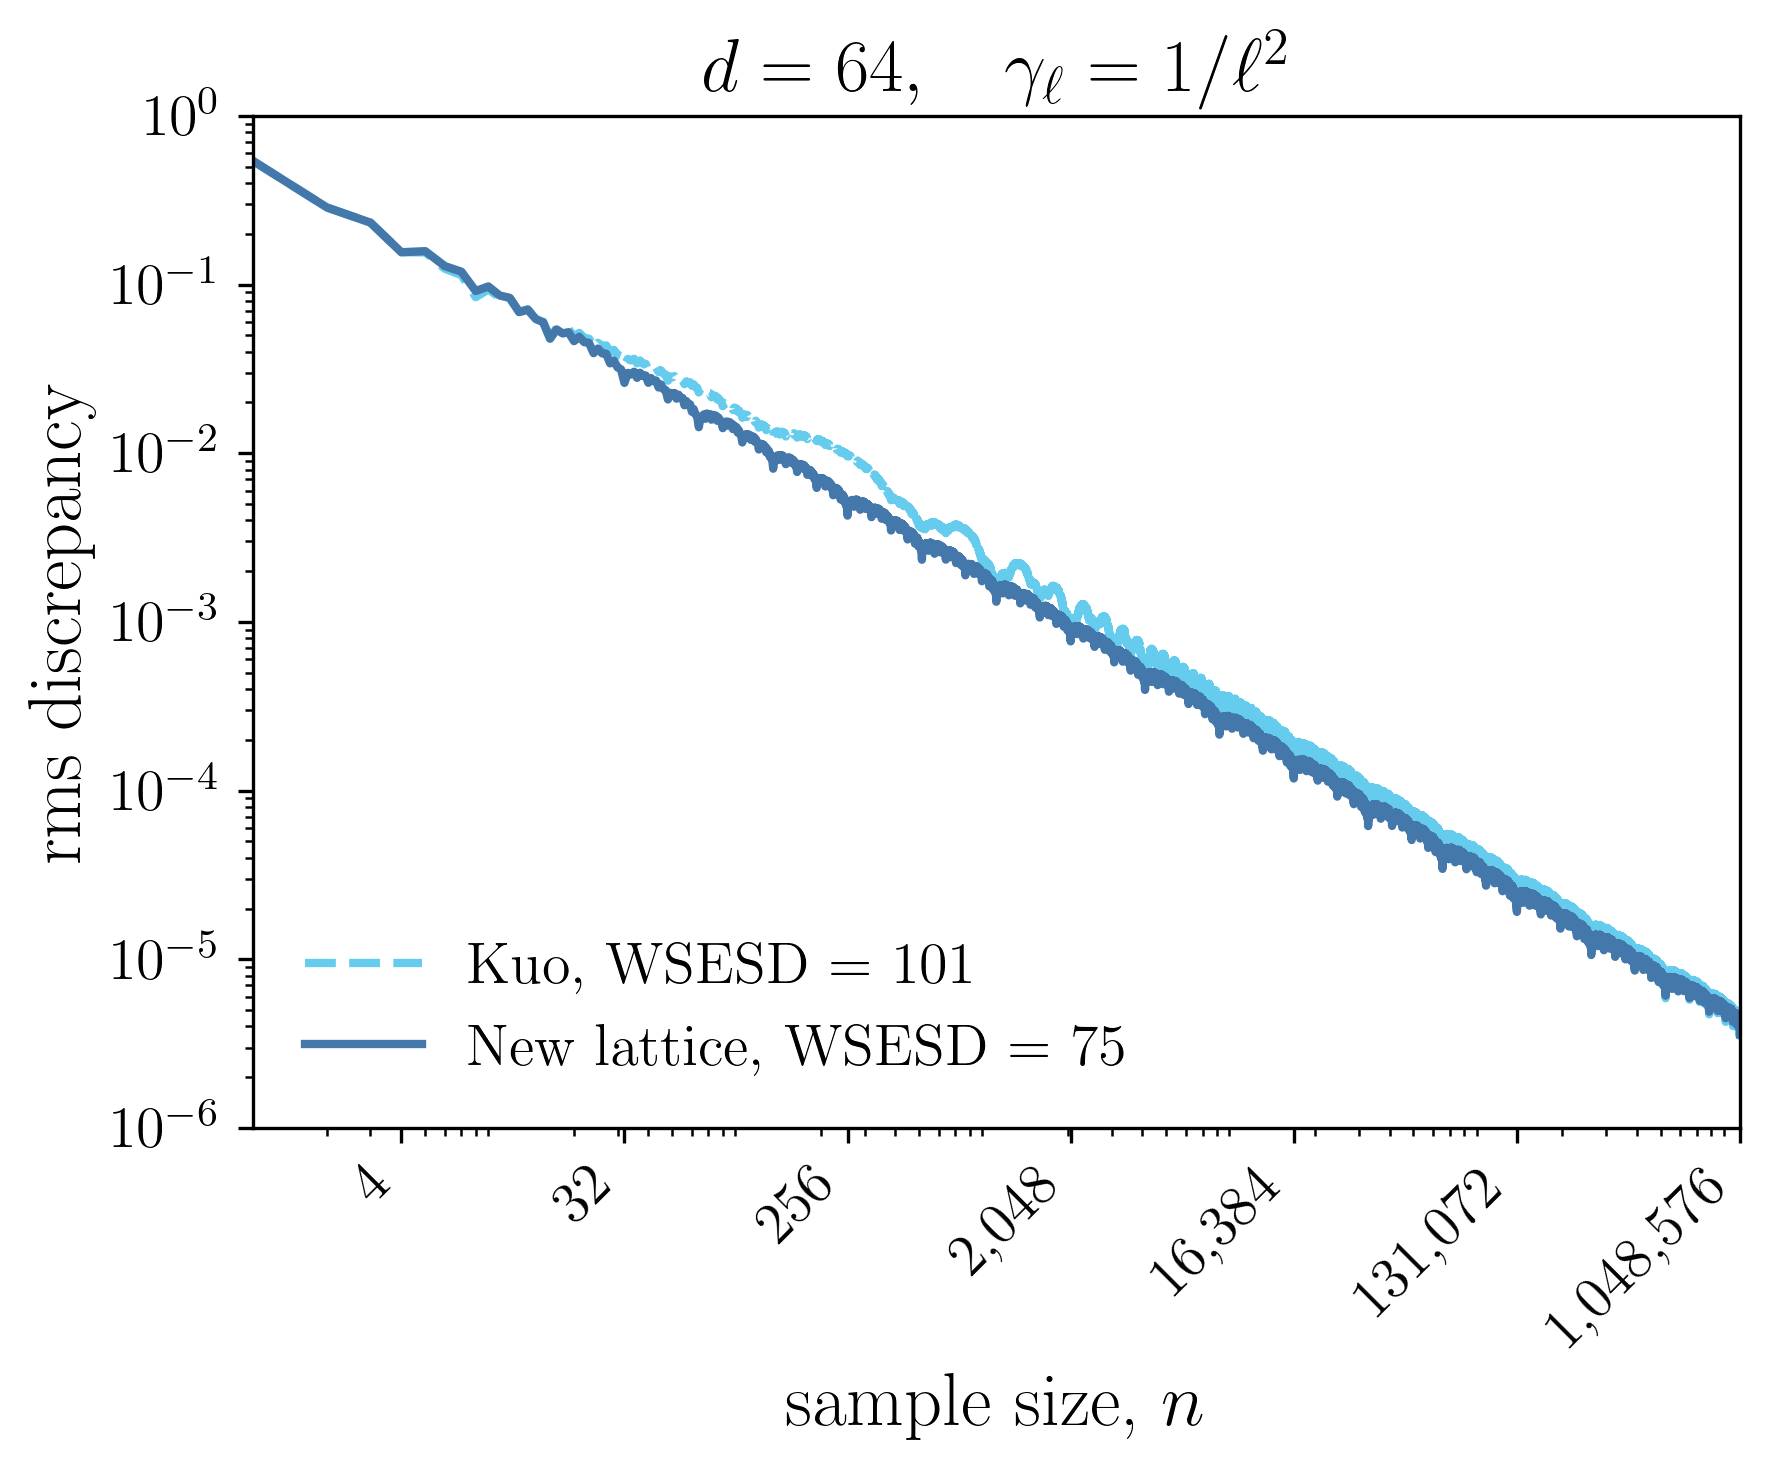
\includegraphics[width=.74\linewidth]{../../notebooks/artifacts/figures/special_d64_lattice_discrepancy.png}\\[1ex]
 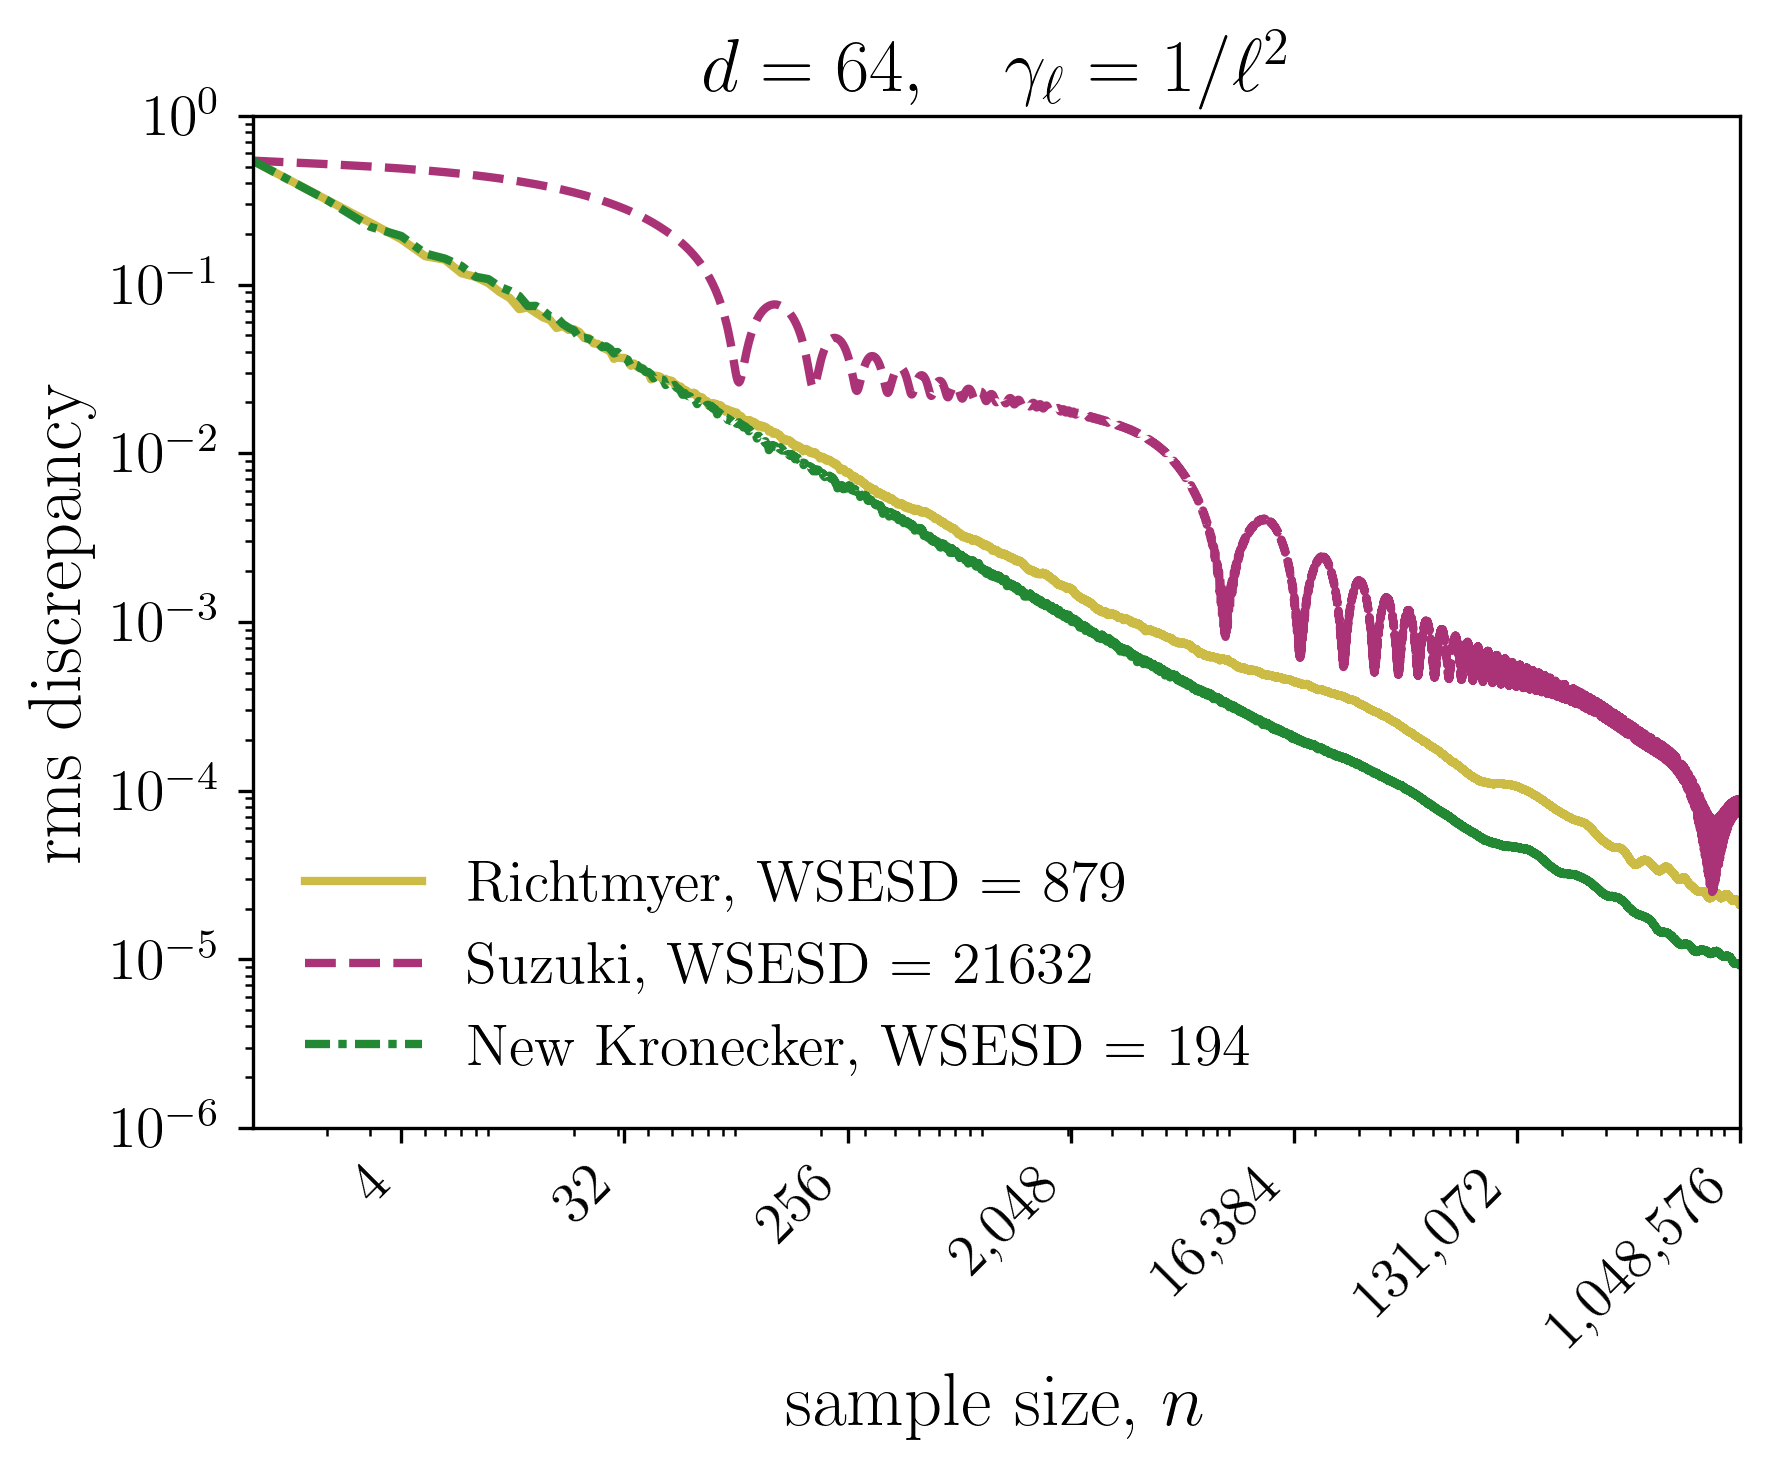
\includegraphics[width=.74\linewidth]{../../notebooks/artifacts/figures/special_d64_kronecker_discrepancy.png}
 \caption{Historical slide illustrations of root expected squared discrepancy:
 lattice sequences (top) and Kronecker sequences (bottom), with $d=64$,
 $N=2^{20}$, $\gamma_j=j^{-2}$, and $w_n=n$. The legends' aggregate values
 are inherited notebook outputs, not newly validated measurements.
 See the accompanying source-provenance record before using them as final results.}
 \label{fig:historical-cbc}
\end{figure}

The initial comparison motivates a more targeted experiment: improvement at
powers of the base need not coincide with improvement of the sum over all
prefix lengths. Conversely, a small aggregate criterion does not imply that
one sequence is best at every $n$. The final experiments should report both
$\W_N$ and the prefix-discrepancy curves, with preferred sample sizes marked,
under the same kernel, weights, and construction horizon.

To test Theorem~\ref{thm:newo-invariance}, fix a generating vector and
compare the original order with several random Newo maps on a finite dyadic
grid. Enumerate scalar pair-difference counts directly, then compare every
prefix's shift-averaged discrepancy with the reduced formula and compare their
weighted sums. The theorem predicts equality for each realized Newo map;
only the uniform-shift expectation remains. For a particular fixed shift or
integrand, integration errors need not agree.

The Kronecker experiments should separately compare the historical CBC rule,
Anders's new rule, and the algebraic baselines. Record the candidate set,
precision, seeds, stopping criteria, generating vectors, construction times,
and software revisions. Start with direct pairwise checks at small $N$ before
using accelerated formulas or reporting large-$N$ results. No new experimental
results are claimed in this draft.

\par\smallskip
\noindent\codex{[Author verification: Revalidate the historical plots before submission. The notebook uses
historical lattice-search interfaces that are absent from the currently pinned
QMCPy source. Also verify that the Kronecker discrepancy routine evaluates the
unshifted differences $\fracpart{k\vz}$: applying a fresh random shift to those
arguments would not implement \eqref{eq:kron-esd}. Inspect the code revision
actually used for the historical figures before drawing a conclusion about
their numerical validity. Agree on the new comparison of CBC methods: common
horizons and weights, intermediate versus preferred sample sizes, construction
costs, and a representative integration example if it fits the page budget.]}
\par\smallskip

\section{Discussion and remaining questions}\label{sec:discussion}
The common design principle is to optimize the prefix curve through a
weighted sum of expected squared discrepancies. For lattice sequences,
dyadic difference multiplicities make this objective tractable. The Newo
invariance result shows that changing the common scalar digit ordering
within the stated class cannot improve this particular criterion for a
fixed generator: every prefix value is already unchanged. Such scrambling
can still change the appearance of a prefix and its integration error for
a particular function. These are separate effects from WSESD optimization.

For Kronecker sequences, the natural decomposition is by integer lags.
It leads to a comparable product-kernel CBC objective, but neither the
lattice search's acceleration nor its available theory transfers merely
because both methods are called CBC. The newer Kronecker construction
should be specified on its own terms, including its candidate family,
search procedure, and finite-horizon or asymptotic guarantees.

The conference abstract proposed arbitrary sample sizes and missing data
as motivations. In this paper, the main results concern all prefixes up to
$N$, whereas~\eqref{eq:removal} gives a limited deletion-stability statement.
A construction specifically optimized over missing-point patterns would
need an additional criterion. Likewise, this draft does not extend the
construction horizon without rebuilding the generator or establish
a stopping rule based on observed integrand values.

\subsection*{Questions for the discussion with Anders}
\codex{[Review agenda for the authors:]}
\codex{\begin{enumerate}[leftmargin=*,itemsep=3pt]
\item Confirm the finite-precision $\pi$ definition and proof in
Section~\ref{sec:newo}, and whether a single infinite-precision family is
needed for the intended implementation.
\item Supply the distinct, newer Kronecker CBC: exact candidate parameters,
objective or surrogate, update rule, cost, and available bounds. Distinguish
it from the \texttt{ANDERS\_CBC} generator used in the talk.
\item Identify a stable implementation and a reproducible figure-generation
path for the lattice and Kronecker searches, including the random-shift
convention in the discrepancy evaluator.
\item Agree on a small numerical study that fits the 16-page limit:
all-prefix comparisons, preferred-size tradeoffs, and a representative
integration example if space permits.
\item Confirm attribution of the new results and the eventual
proceedings format before submission.
\end{enumerate}
These questions identify work remaining in the draft rather than claims
that the numerical results or the newer algorithm have already been verified.}

\bibliographystyle{spmpsci}
\bibliography{references}
\end{document}
